\documentclass[tikz,border=4pt]{standalone}
\usepackage[T1]{fontenc}
\usepackage{lmodern}
\usepackage{amsmath}
% Shared TikZ style for the report figures.
% Colours follow the Okabe-Ito palette, which stays distinguishable under the
% common forms of colour-vision deficiency. Every colour-coded element also
% carries a text label, so no figure depends on colour alone.
\usetikzlibrary{arrows.meta,positioning,fit,calc,backgrounds,decorations.pathreplacing,shapes.geometric}

\definecolor{oiOrange}{HTML}{E69F00}
\definecolor{oiSky}{HTML}{56B4E9}
\definecolor{oiGreen}{HTML}{009E73}
\definecolor{oiYellow}{HTML}{F0E442}
\definecolor{oiBlue}{HTML}{0072B2}
\definecolor{oiVerm}{HTML}{D55E00}
\definecolor{oiPurple}{HTML}{CC79A7}
\definecolor{oiGray}{HTML}{6E6E6E}

\colorlet{corTreino}{oiBlue!22}
\colorlet{corValid}{oiGreen!30}
\colorlet{corTeste}{oiOrange!45}
\colorlet{corControle}{oiPurple!35}

\tikzset{
  >=Stealth,
  bloco/.style={draw=black!70, rounded corners=1.5pt, minimum height=0.62cm,
    inner sep=2pt, font=\sffamily\fsz, align=center},
  treino/.style={bloco, fill=corTreino},
  valid/.style={bloco, fill=corValid},
  teste/.style={bloco, fill=corTeste, thick},
  etapa/.style={draw=black!70, rounded corners=3pt, fill=black!4,
    text width=4.3cm, align=center, inner sep=4pt, font=\sffamily\fsz},
  nota/.style={font=\sffamily\fsz, align=left, text=black!80},
  titulo/.style={font=\sffamily\fst\bfseries, anchor=west},
  seta/.style={->, thick, black!70},
  regiao/.style={draw=black!50, dashed, rounded corners=4pt},
}

% Absolute font sizes, so a figure looks the same standalone (10 pt class) and
% inside the 11 pt report.
\providecommand{\fsx}{\fontsize{5.5}{6.5}\selectfont}
\providecommand{\fsz}{\fontsize{7}{8.5}\selectfont}
\providecommand{\fst}{\fontsize{9}{11}\selectfont}

\begin{document}
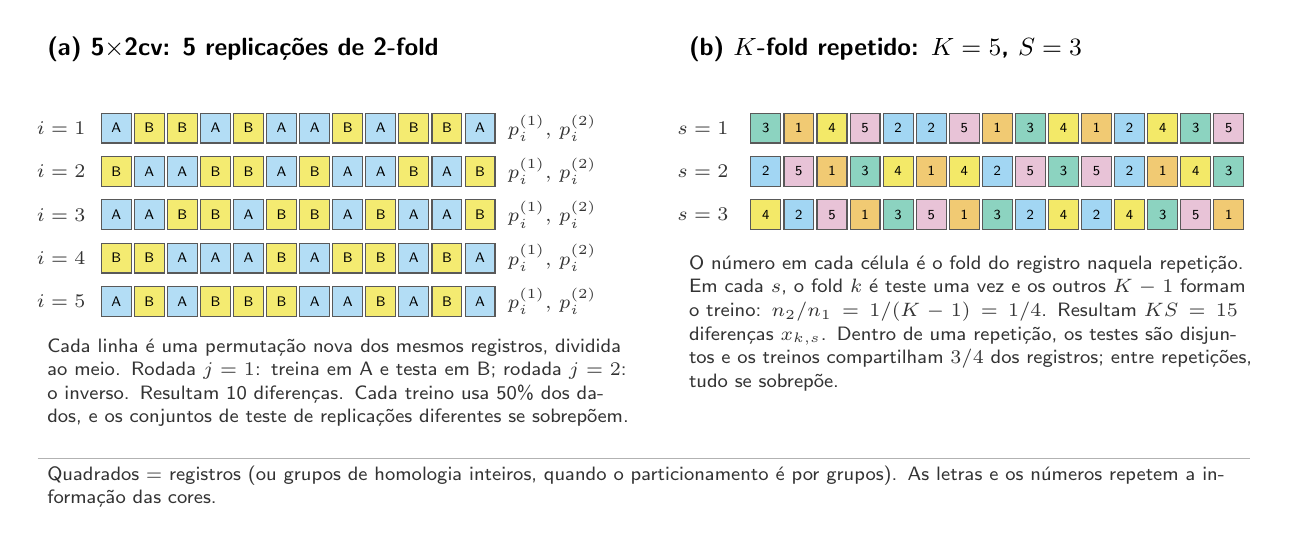
\begin{tikzpicture}[
  cel/.style={draw=black!65, minimum size=0.38cm, inner sep=0pt, font=\sffamily\fsx},
  ]
  % ---------------- (a) 5x2cv ----------------
  \node[titulo] at (0,0.45) {(a) 5$\times$2cv: 5 replicações de 2-fold};
  \foreach \i/\row in {1/{A,B,B,A,B,A,A,B,A,B,B,A},
                       2/{B,A,A,B,B,A,B,A,A,B,A,B},
                       3/{A,A,B,B,A,B,B,A,B,A,A,B},
                       4/{B,B,A,A,A,B,A,B,B,A,B,A},
                       5/{A,B,A,B,B,B,A,A,B,A,B,A}} {
    \pgfmathsetmacro\y{-0.55*\i}
    \node[nota] at (0.3,\y) {$i=\i$};
    \foreach \v [count=\c] in \row {
      \pgfmathsetmacro\x{1.0+0.42*(\c-1)}
      \if\v A \node[cel, fill=oiSky!45] at (\x,\y) {A};
      \else   \node[cel, fill=oiYellow!75] at (\x,\y) {B}; \fi
    }
    \node[nota, anchor=west] at (5.85,\y) {$p_i^{(1)},\,p_i^{(2)}$};
  }
  \node[nota, text width=7.4cm, anchor=north west] at (0,-3.1)
    {Cada linha é uma permutação nova dos mesmos registros, dividida ao meio. Rodada $j=1$: treina em A e testa em B; rodada $j=2$: o inverso. Resultam 10 diferenças. Cada treino usa 50\% dos dados, e os conjuntos de teste de replicações diferentes se sobrepõem.};

  % ---------------- (b) repeated K-fold ----------------
  \node[titulo] at (8.15,0.45) {(b) $K$-fold repetido: $K=5$, $S=3$};
  \foreach \s/\row in {1/{3,1,4,5,2,2,5,1,3,4,1,2,4,3,5},
                       2/{2,5,1,3,4,1,4,2,5,3,5,2,1,4,3},
                       3/{4,2,5,1,3,5,1,3,2,4,2,4,3,5,1}} {
    \pgfmathsetmacro\y{-0.55*\s}
    \node[nota] at (8.45,\y) {$s=\s$};
    \foreach \v [count=\c] in \row {
      \pgfmathsetmacro\x{9.25+0.42*(\c-1)}
      \ifcase\v\or
        \node[cel, fill=oiOrange!55] at (\x,\y) {\v};\or
        \node[cel, fill=oiSky!55] at (\x,\y) {\v};\or
        \node[cel, fill=oiGreen!45] at (\x,\y) {\v};\or
        \node[cel, fill=oiYellow!80] at (\x,\y) {\v};\or
        \node[cel, fill=oiPurple!45] at (\x,\y) {\v};\fi
    }
  }
  \node[nota, text width=7.3cm, anchor=north west] at (8.15,-2.05)
    {O número em cada célula é o fold do registro naquela repetição. Em cada $s$, o fold $k$ é teste uma vez e os outros $K-1$ formam o treino: $n_2/n_1 = 1/(K-1) = 1/4$. Resultam $KS=15$ diferenças $x_{k,s}$. Dentro de uma repetição, os testes são disjuntos e os treinos compartilham $3/4$ dos registros; entre repetições, tudo se sobrepõe.};

  % ---------------- shared caption strip ----------------
  \draw[black!30] (0,-4.75) -- (15.4,-4.75);
  \node[nota, anchor=west, text width=15.3cm] at (0,-5.1)
    {Quadrados = registros (ou grupos de homologia inteiros, quando o particionamento é por grupos). As letras e os números repetem a informação das cores.};
\end{tikzpicture}
\end{document}
